\documentclass[tikz,border=0pt]{standalone}
\usepackage[T1]{fontenc}
\usepackage{newtxtext,newtxmath}
\usepackage{xcolor}
\definecolor{blue}{HTML}{326C9B}
\definecolor{gray}{HTML}{75818D}
\definecolor{ink}{HTML}{203244}
\definecolor{grid}{HTML}{E6EAF0}
\definecolor{yellow}{HTML}{FFF19A}
\begin{document}
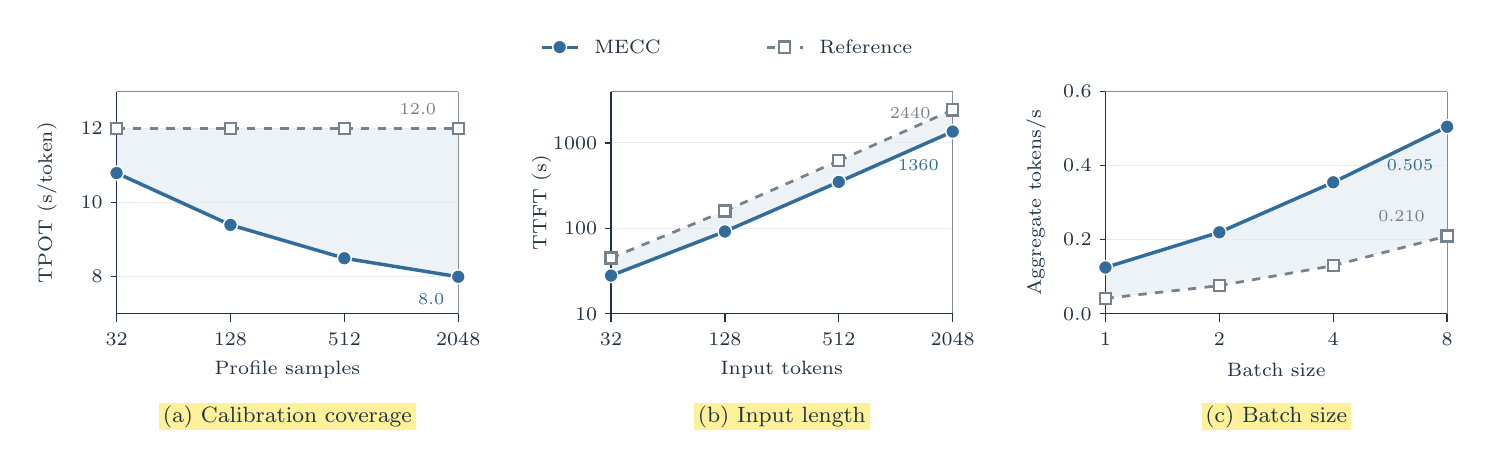
\begin{tikzpicture}[x=1bp,y=-1bp,every node/.style={inner sep=0pt,outer sep=0pt,text=ink,font=\fontsize{7.2}{8.2}\selectfont}]
\path[use as bounding box] (0,0) rectangle (522,148);
\draw[blue,line width=1.15bp] (185.000,7.000)--(198.000,7.000);
\filldraw[fill=blue,draw=white,line width=.5bp] (191.500,7.000) circle[radius=2.5bp];
\node[anchor=west,text=ink,font=\fontsize{7}{8}\selectfont] at (204.000,7.000) {MECC};
\draw[gray,line width=1bp,dashed] (266.000,7.000)--(279.000,7.000);
\filldraw[fill=white,draw=gray,line width=.8bp] (270.500,5.000) rectangle (274.500,9.000);
\node[anchor=west,text=ink,font=\fontsize{7}{8}\selectfont] at (285.000,7.000) {Reference};
\fill[blue!9] (32.000,36.333)--(73.000,36.333)--(114.000,36.333)--(155.000,36.333)--(155.000,89.667)--(114.000,83.000)--(73.000,71.000)--(32.000,52.333)--cycle;
\draw[grid,line width=0.35bp] (32.000,89.667)--(155.000,89.667);
\draw[ink,line width=0.45bp] (30.000,89.667)--(32.000,89.667);
\node[anchor=east,text=ink,font=\fontsize{6.7}{7.7}\selectfont] at (27.000,89.667) {8};
\draw[grid,line width=0.35bp] (32.000,63.000)--(155.000,63.000);
\draw[ink,line width=0.45bp] (30.000,63.000)--(32.000,63.000);
\node[anchor=east,text=ink,font=\fontsize{6.7}{7.7}\selectfont] at (27.000,63.000) {10};
\draw[grid,line width=0.35bp] (32.000,36.333)--(155.000,36.333);
\draw[ink,line width=0.45bp] (30.000,36.333)--(32.000,36.333);
\node[anchor=east,text=ink,font=\fontsize{6.7}{7.7}\selectfont] at (27.000,36.333) {12};
\draw[ink!55,line width=0.4bp] (32.000,23.000)--(155.000,23.000);
\draw[ink!55,line width=0.4bp] (155.000,23.000)--(155.000,103.000);
\draw[ink,line width=0.5bp] (32.000,23.000)--(32.000,103.000);
\draw[ink,line width=0.5bp] (32.000,103.000)--(155.000,103.000);
\draw[gray,line width=1bp,dashed] (32.000,36.333)--(73.000,36.333);
\draw[gray,line width=1bp,dashed] (73.000,36.333)--(114.000,36.333);
\draw[gray,line width=1bp,dashed] (114.000,36.333)--(155.000,36.333);
\filldraw[fill=white,draw=gray,line width=.8bp] (30.000,34.333) rectangle (34.000,38.333);
\filldraw[fill=white,draw=gray,line width=.8bp] (71.000,34.333) rectangle (75.000,38.333);
\filldraw[fill=white,draw=gray,line width=.8bp] (112.000,34.333) rectangle (116.000,38.333);
\filldraw[fill=white,draw=gray,line width=.8bp] (153.000,34.333) rectangle (157.000,38.333);
\draw[blue,line width=1.25bp] (32.000,52.333)--(73.000,71.000);
\draw[blue,line width=1.25bp] (73.000,71.000)--(114.000,83.000);
\draw[blue,line width=1.25bp] (114.000,83.000)--(155.000,89.667);
\filldraw[fill=blue,draw=white,line width=.5bp] (32.000,52.333) circle[radius=2.5bp];
\filldraw[fill=blue,draw=white,line width=.5bp] (73.000,71.000) circle[radius=2.5bp];
\filldraw[fill=blue,draw=white,line width=.5bp] (114.000,83.000) circle[radius=2.5bp];
\filldraw[fill=blue,draw=white,line width=.5bp] (155.000,89.667) circle[radius=2.5bp];
\draw[ink,line width=0.45bp] (32.000,103.000)--(32.000,106.000);
\node[anchor=center,text=ink,font=\fontsize{6.7}{7.7}\selectfont] at (32.000,112.000) {32};
\draw[ink,line width=0.45bp] (73.000,103.000)--(73.000,106.000);
\node[anchor=center,text=ink,font=\fontsize{6.7}{7.7}\selectfont] at (73.000,112.000) {128};
\draw[ink,line width=0.45bp] (114.000,103.000)--(114.000,106.000);
\node[anchor=center,text=ink,font=\fontsize{6.7}{7.7}\selectfont] at (114.000,112.000) {512};
\draw[ink,line width=0.45bp] (155.000,103.000)--(155.000,106.000);
\node[anchor=center,text=ink,font=\fontsize{6.7}{7.7}\selectfont] at (155.000,112.000) {2048};
\node[anchor=center,text=ink,font=\fontsize{7.2}{8.2}\selectfont,rotate=90] at (7.000,63.000) {TPOT (s/token)};
\node[anchor=center,text=ink,font=\fontsize{7.2}{8.2}\selectfont] at (93.500,123.000) {Profile samples};
\node[anchor=center,text=ink,font=\fontsize{7.8}{8.8}\selectfont,fill=yellow,inner xsep=1.4bp,inner ysep=1.0bp] at (93.500,140.000) {(a) Calibration coverage};
\node[anchor=east,text=gray,font=\fontsize{6.5}{7.5}\selectfont] at (147.000,29.333) {12.0};
\node[anchor=east,text=blue,font=\fontsize{6.5}{7.5}\selectfont] at (150.000,97.667) {8.0};
\fill[blue!9] (210.000,82.917)--(251.000,65.979)--(292.000,47.893)--(333.000,29.600)--(333.000,37.405)--(292.000,55.528)--(251.000,73.368)--(210.000,89.252)--cycle;
\draw[grid,line width=0.35bp] (210.000,103.000)--(333.000,103.000);
\draw[ink,line width=0.45bp] (208.000,103.000)--(210.000,103.000);
\node[anchor=east,text=ink,font=\fontsize{6.7}{7.7}\selectfont] at (205.000,103.000) {10};
\draw[grid,line width=0.35bp] (210.000,72.255)--(333.000,72.255);
\draw[ink,line width=0.45bp] (208.000,72.255)--(210.000,72.255);
\node[anchor=east,text=ink,font=\fontsize{6.7}{7.7}\selectfont] at (205.000,72.255) {100};
\draw[grid,line width=0.35bp] (210.000,41.510)--(333.000,41.510);
\draw[ink,line width=0.45bp] (208.000,41.510)--(210.000,41.510);
\node[anchor=east,text=ink,font=\fontsize{6.7}{7.7}\selectfont] at (205.000,41.510) {1000};
\draw[ink!55,line width=0.4bp] (210.000,23.000)--(333.000,23.000);
\draw[ink!55,line width=0.4bp] (333.000,23.000)--(333.000,103.000);
\draw[ink,line width=0.5bp] (210.000,23.000)--(210.000,103.000);
\draw[ink,line width=0.5bp] (210.000,103.000)--(333.000,103.000);
\draw[gray,line width=1bp,dashed] (210.000,82.917)--(251.000,65.979);
\draw[gray,line width=1bp,dashed] (251.000,65.979)--(292.000,47.893);
\draw[gray,line width=1bp,dashed] (292.000,47.893)--(333.000,29.600);
\filldraw[fill=white,draw=gray,line width=.8bp] (208.000,80.917) rectangle (212.000,84.917);
\filldraw[fill=white,draw=gray,line width=.8bp] (249.000,63.979) rectangle (253.000,67.979);
\filldraw[fill=white,draw=gray,line width=.8bp] (290.000,45.893) rectangle (294.000,49.893);
\filldraw[fill=white,draw=gray,line width=.8bp] (331.000,27.600) rectangle (335.000,31.600);
\draw[blue,line width=1.25bp] (210.000,89.252)--(251.000,73.368);
\draw[blue,line width=1.25bp] (251.000,73.368)--(292.000,55.528);
\draw[blue,line width=1.25bp] (292.000,55.528)--(333.000,37.405);
\filldraw[fill=blue,draw=white,line width=.5bp] (210.000,89.252) circle[radius=2.5bp];
\filldraw[fill=blue,draw=white,line width=.5bp] (251.000,73.368) circle[radius=2.5bp];
\filldraw[fill=blue,draw=white,line width=.5bp] (292.000,55.528) circle[radius=2.5bp];
\filldraw[fill=blue,draw=white,line width=.5bp] (333.000,37.405) circle[radius=2.5bp];
\draw[ink,line width=0.45bp] (210.000,103.000)--(210.000,106.000);
\node[anchor=center,text=ink,font=\fontsize{6.7}{7.7}\selectfont] at (210.000,112.000) {32};
\draw[ink,line width=0.45bp] (251.000,103.000)--(251.000,106.000);
\node[anchor=center,text=ink,font=\fontsize{6.7}{7.7}\selectfont] at (251.000,112.000) {128};
\draw[ink,line width=0.45bp] (292.000,103.000)--(292.000,106.000);
\node[anchor=center,text=ink,font=\fontsize{6.7}{7.7}\selectfont] at (292.000,112.000) {512};
\draw[ink,line width=0.45bp] (333.000,103.000)--(333.000,106.000);
\node[anchor=center,text=ink,font=\fontsize{6.7}{7.7}\selectfont] at (333.000,112.000) {2048};
\node[anchor=center,text=ink,font=\fontsize{7.2}{8.2}\selectfont,rotate=90] at (185.000,63.000) {TTFT (s)};
\node[anchor=center,text=ink,font=\fontsize{7.2}{8.2}\selectfont] at (271.500,123.000) {Input tokens};
\node[anchor=center,text=ink,font=\fontsize{7.8}{8.8}\selectfont,fill=yellow,inner xsep=1.4bp,inner ysep=1.0bp] at (271.500,140.000) {(b) Input length};
\node[anchor=east,text=gray,font=\fontsize{6.5}{7.5}\selectfont] at (325.000,30.600) {2440};
\node[anchor=east,text=blue,font=\fontsize{6.5}{7.5}\selectfont] at (328.000,49.405) {1360};
\fill[blue!9] (388.000,97.444)--(429.000,92.867)--(470.000,85.667)--(511.000,75.000)--(511.000,35.667)--(470.000,55.667)--(429.000,73.667)--(388.000,86.333)--cycle;
\draw[grid,line width=0.35bp] (388.000,103.000)--(511.000,103.000);
\draw[ink,line width=0.45bp] (386.000,103.000)--(388.000,103.000);
\node[anchor=east,text=ink,font=\fontsize{6.7}{7.7}\selectfont] at (383.000,103.000) {0.0};
\draw[grid,line width=0.35bp] (388.000,76.333)--(511.000,76.333);
\draw[ink,line width=0.45bp] (386.000,76.333)--(388.000,76.333);
\node[anchor=east,text=ink,font=\fontsize{6.7}{7.7}\selectfont] at (383.000,76.333) {0.2};
\draw[grid,line width=0.35bp] (388.000,49.667)--(511.000,49.667);
\draw[ink,line width=0.45bp] (386.000,49.667)--(388.000,49.667);
\node[anchor=east,text=ink,font=\fontsize{6.7}{7.7}\selectfont] at (383.000,49.667) {0.4};
\draw[grid,line width=0.35bp] (388.000,23.000)--(511.000,23.000);
\draw[ink,line width=0.45bp] (386.000,23.000)--(388.000,23.000);
\node[anchor=east,text=ink,font=\fontsize{6.7}{7.7}\selectfont] at (383.000,23.000) {0.6};
\draw[ink!55,line width=0.4bp] (388.000,23.000)--(511.000,23.000);
\draw[ink!55,line width=0.4bp] (511.000,23.000)--(511.000,103.000);
\draw[ink,line width=0.5bp] (388.000,23.000)--(388.000,103.000);
\draw[ink,line width=0.5bp] (388.000,103.000)--(511.000,103.000);
\draw[gray,line width=1bp,dashed] (388.000,97.444)--(429.000,92.867);
\draw[gray,line width=1bp,dashed] (429.000,92.867)--(470.000,85.667);
\draw[gray,line width=1bp,dashed] (470.000,85.667)--(511.000,75.000);
\filldraw[fill=white,draw=gray,line width=.8bp] (386.000,95.444) rectangle (390.000,99.444);
\filldraw[fill=white,draw=gray,line width=.8bp] (427.000,90.867) rectangle (431.000,94.867);
\filldraw[fill=white,draw=gray,line width=.8bp] (468.000,83.667) rectangle (472.000,87.667);
\filldraw[fill=white,draw=gray,line width=.8bp] (509.000,73.000) rectangle (513.000,77.000);
\draw[blue,line width=1.25bp] (388.000,86.333)--(429.000,73.667);
\draw[blue,line width=1.25bp] (429.000,73.667)--(470.000,55.667);
\draw[blue,line width=1.25bp] (470.000,55.667)--(511.000,35.667);
\filldraw[fill=blue,draw=white,line width=.5bp] (388.000,86.333) circle[radius=2.5bp];
\filldraw[fill=blue,draw=white,line width=.5bp] (429.000,73.667) circle[radius=2.5bp];
\filldraw[fill=blue,draw=white,line width=.5bp] (470.000,55.667) circle[radius=2.5bp];
\filldraw[fill=blue,draw=white,line width=.5bp] (511.000,35.667) circle[radius=2.5bp];
\draw[ink,line width=0.45bp] (388.000,103.000)--(388.000,106.000);
\node[anchor=center,text=ink,font=\fontsize{6.7}{7.7}\selectfont] at (388.000,112.000) {1};
\draw[ink,line width=0.45bp] (429.000,103.000)--(429.000,106.000);
\node[anchor=center,text=ink,font=\fontsize{6.7}{7.7}\selectfont] at (429.000,112.000) {2};
\draw[ink,line width=0.45bp] (470.000,103.000)--(470.000,106.000);
\node[anchor=center,text=ink,font=\fontsize{6.7}{7.7}\selectfont] at (470.000,112.000) {4};
\draw[ink,line width=0.45bp] (511.000,103.000)--(511.000,106.000);
\node[anchor=center,text=ink,font=\fontsize{6.7}{7.7}\selectfont] at (511.000,112.000) {8};
\node[anchor=center,text=ink,font=\fontsize{7.2}{8.2}\selectfont,rotate=90] at (363.000,63.000) {Aggregate tokens/s};
\node[anchor=center,text=ink,font=\fontsize{7.2}{8.2}\selectfont] at (449.500,123.000) {Batch size};
\node[anchor=center,text=ink,font=\fontsize{7.8}{8.8}\selectfont,fill=yellow,inner xsep=1.4bp,inner ysep=1.0bp] at (449.500,140.000) {(c) Batch size};
\node[anchor=east,text=gray,font=\fontsize{6.5}{7.5}\selectfont] at (503.000,68.000) {0.210};
\node[anchor=east,text=blue,font=\fontsize{6.5}{7.5}\selectfont] at (506.000,49.667) {0.505};
\end{tikzpicture}
\end{document}
